%%%%%%%%%%%%%%%%%%%%%%%%%%%%%%%%%%%%%%%%
% datoteka diploma-vzorec.tex
%
% vzorčna datoteka za pisanje diplomskega dela v formatu LaTeX
% na UL Fakulteti za računalništvo in informatiko
%
% vkup spravil Gašper Fijavž, december 2010
% 
%
%
% verzija 12. februar 2014 (besedilo teme, seznam kratic, popravki Gašper Fijavž)
% verzija 10. marec 2014 (redakcijski popravki Zoran Bosnić)
% verzija 11. marec 2014 (redakcijski popravki Gašper Fijavž)
% verzija 15. april 2014 (pdf/a 1b compliance, not really - just claiming, Damjan Cvetan, Gašper Fijavž)
% verzija 23. april 2014 (privzeto cc licenca)
% verzija 16. september 2014 (odmiki strain od roba)
% verzija 28. oktober 2014 (odstranil vpisno številko)
% verija 5. februar 2015 (Literatura v kazalu, online literatura)

\documentclass[a4paper, 12pt]{book}

\usepackage[utf8x]{inputenc}   % omogoča uporabo slovenskih črk kodiranih v formatu UTF-8
\usepackage[slovene,english]{babel}    % naloži, med drugim, slovenske delilne vzorce
\usepackage[pdftex]{graphicx}  % omogoča vlaganje slik različnih formatov
\usepackage{fancyhdr}          % poskrbi, na primer, za glave strani
\usepackage{amssymb}           % dodatni simboli
\usepackage{amsmath}           % eqref, npr.
\usepackage{float}
\usepackage{listings}
%\usepackage{hyperxmp}
\usepackage[pdftex, colorlinks=true,
						citecolor=black, filecolor=black, 
						linkcolor=black, urlcolor=black,
						pagebackref=false, 
						pdfproducer={LaTeX}, pdfcreator={LaTeX}, hidelinks]{hyperref}


%%%%%%%%%%%%%%%%%%%%%%%%%%%%%%%%%%%%%%%%
%	DIPLOMA INFO
%%%%%%%%%%%%%%%%%%%%%%%%%%%%%%%%%%%%%%%%
\newcommand{\ttitle}{Generiranje svetlobi prilagonjenih dreves z uporabo genetskih algoritmov}
\newcommand{\ttitleEn}{Generation of light source adapted tree models with the use of genetic algorithms}
\newcommand{\tsubject}{\ttitle}
\newcommand{\tsubjectEn}{\ttitleEn}
\newcommand{\tauthor}{Juš Lozej}
\newcommand{\tkeywords}{računalnik, računalnik, računalnik}
\newcommand{\tkeywordsEn}{computer, computer, computer}



\usepackage{hyperref}
%%%%%%%%%%%%%%%%%%%%%%%%%%%%%%%%%%%%%%%%
%	HYPERREF SETUP
%%%%%%%%%%%%%%%%%%%%%%%%%%%%%%%%%%%%%%%%
\hypersetup{pdftitle={\ttitle}}
\hypersetup{pdfsubject=\ttitleEn}
\hypersetup{pdfauthor={\tauthor, jlozej@gmail.com}}
\hypersetup{pdfkeywords=\tkeywordsEn}


 


%%%%%%%%%%%%%%%%%%%%%%%%%%%%%%%%%%%%%%%%
% postavitev strani
%%%%%%%%%%%%%%%%%%%%%%%%%%%%%%%%%%%%%%%%  

\addtolength{\marginparwidth}{-20pt} % robovi za tisk
\addtolength{\oddsidemargin}{40pt}
\addtolength{\evensidemargin}{-40pt}

\renewcommand{\baselinestretch}{1.3} % ustrezen razmik med vrsticami
\setlength{\headheight}{15pt}        % potreben prostor na vrhu
\renewcommand{\chaptermark}[1]%
{\markboth{\MakeUppercase{\thechapter.\ #1}}{}} \renewcommand{\sectionmark}[1]%
{\markright{\MakeUppercase{\thesection.\ #1}}} \renewcommand{\headrulewidth}{0.5pt} \renewcommand{\footrulewidth}{0pt}
\fancyhf{}
\fancyhead[LE,RO]{\sl \thepage} \fancyhead[LO]{\sl \rightmark} \fancyhead[RE]{\sl \leftmark}



\newcommand{\BibTeX}{{\sc Bib}\TeX}

%%%%%%%%%%%%%%%%%%%%%%%%%%%%%%%%%%%%%%%%
% naslovi
%%%%%%%%%%%%%%%%%%%%%%%%%%%%%%%%%%%%%%%%  


\newcommand{\autfont}{\Large}
\newcommand{\titfont}{\LARGE\bf}
\newcommand{\clearemptydoublepage}{\newpage{\pagestyle{empty}\cleardoublepage}}
\setcounter{tocdepth}{1}	      % globina kazala

%%%%%%%%%%%%%%%%%%%%%%%%%%%%%%%%%%%%%%%%
% konstrukti
%%%%%%%%%%%%%%%%%%%%%%%%%%%%%%%%%%%%%%%%  
\newtheorem{izrek}{Izrek}[chapter]
\newtheorem{trditev}{Trditev}[izrek]
\newenvironment{dokaz}{\emph{Dokaz.}\ }{\hspace{\fill}{$\Box$}}

%%%%%%%%%%%%%%%%%%%%%%%%%%%%%%%%%%%%%%%%%%%%%%%%%%%%%%%%%%%%%%%%%%%%%%%%%%%%%%%
%% PDF-A
%%%%%%%%%%%%%%%%%%%%%%%%%%%%%%%%%%%%%%%%%%%%%%%%%%%%%%%%%%%%%%%%%%%%%%%%%%%%%%%

%%%%%%%%%%%%%%%%%%%%%%%%%%%%%%%%%%%%%%%% 
% define medatata
%%%%%%%%%%%%%%%%%%%%%%%%%%%%%%%%%%%%%%%% 
\def\Title{\ttitle}
\def\Author{\tauthor, jlozej@gmail.com}
\def\Subject{\ttitleEn}
\def\Keywords{\tkeywordsEn}

%%%%%%%%%%%%%%%%%%%%%%%%%%%%%%%%%%%%%%%% 
% \convertDate converts D:20080419103507+02'00' to 2008-04-19T10:35:07+02:00
%%%%%%%%%%%%%%%%%%%%%%%%%%%%%%%%%%%%%%%% 
\def\convertDate{%
    \getYear
}

{\catcode`\D=12
 \gdef\getYear D:#1#2#3#4{\edef\xYear{#1#2#3#4}\getMonth}
}
\def\getMonth#1#2{\edef\xMonth{#1#2}\getDay}
\def\getDay#1#2{\edef\xDay{#1#2}\getHour}
\def\getHour#1#2{\edef\xHour{#1#2}\getMin}
\def\getMin#1#2{\edef\xMin{#1#2}\getSec}
\def\getSec#1#2{\edef\xSec{#1#2}\getTZh}
\def\getTZh +#1#2{\edef\xTZh{#1#2}\getTZm}
\def\getTZm '#1#2'{%
    \edef\xTZm{#1#2}%
    \edef\convDate{\xYear-\xMonth-\xDay T\xHour:\xMin:\xSec+\xTZh:\xTZm}%
}

\expandafter\convertDate\pdfcreationdate 

%%%%%%%%%%%%%%%%%%%%%%%%%%%%%%%%%%%%%%%%
% get pdftex version string
%%%%%%%%%%%%%%%%%%%%%%%%%%%%%%%%%%%%%%%% 
\newcount\countA
\countA=\pdftexversion
\advance \countA by -100
\def\pdftexVersionStr{pdfTeX-1.\the\countA.\pdftexrevision}


%%%%%%%%%%%%%%%%%%%%%%%%%%%%%%%%%%%%%%%%
% XMP data
%%%%%%%%%%%%%%%%%%%%%%%%%%%%%%%%%%%%%%%%  
\usepackage{xmpincl}
\includexmp{pdfa-1b}

%%%%%%%%%%%%%%%%%%%%%%%%%%%%%%%%%%%%%%%%
% pdfInfo
%%%%%%%%%%%%%%%%%%%%%%%%%%%%%%%%%%%%%%%%  
\pdfinfo{%
    /Title    (\ttitle)
    /Author   (\tauthor, damjan@cvetan.si)
    /Subject  (\ttitleEn)
    /Keywords (\tkeywordsEn)
    /ModDate  (\pdfcreationdate)
    /Trapped  /False
}


%%%%%%%%%%%%%%%%%%%%%%%%%%%%%%%%%%%%%%%%%%%%%%%%%%%%%%%%%%%%%%%%%%%%%%%%%%%%%%%
%%%%%%%%%%%%%%%%%%%%%%%%%%%%%%%%%%%%%%%%%%%%%%%%%%%%%%%%%%%%%%%%%%%%%%%%%%%%%%%

\begin{document}
\selectlanguage{slovene}
\frontmatter
\setcounter{page}{1} %
\renewcommand{\thepage}{}       % preprecimo težave s številkami strani v kazalu

%%%%%%%%%%%%%%%%%%%%%%%%%%%%%%%%%%%%%%%%
%naslovnica
 \thispagestyle{empty}%
   \begin{center}
    {\large\sc Univerza v Ljubljani\\%
      Fakulteta za računalništvo in informatiko}%
    \vskip 10em%
    {\autfont \tauthor\par}%
    {\titfont \ttitle \par}%
    {\vskip 2em \textsc{DIPLOMSKO DELO\\[2mm]
    UNIVERZITETNI ŠTUDIJSKI PROGRAM PRVE STOPNJE
RAČUNALNISTVO IN INFORMATIKA}\par}%
    \vfill\null%
    {\large \textsc{Mentor}: prof.\ dr.  Marko Bajec\par}%
    {\vskip 2em \large Ljubljana 2015 \par}%
\end{center}
% prazna stran
\clearemptydoublepage

%%%%%%%%%%%%%%%%%%%%%%%%%%%%%%%%%%%%%%%%
%copyright stran
\thispagestyle{empty}
\vspace*{8cm}
Fakulteta za računalništvo in informatiko podpira javno dostopnost znanstvenih, strokovnih in razvojnih rezultatov. Zato priporoča objavo dela pod katero od licenc, ki omogočajo prosto razširjanje diplomskega dela in/ali možnost nadaljne proste uporabe dela. Ena izmed možnosti je izdaja diplomskega dela pod katero od Creative Commons licenc \href{http://creativecommons.si}{http://creativecommons.si}

Morebitno pripadajočo programsko kodo praviloma objavite pod, denimo, licenco 
\emph{GNU General Public License, različica 3}. Podrobnosti licence so dostopne na spletni strani \href{http://www.gnu.org/licenses/}{http://www.gnu.org/licenses/}.

\begin{center}
\mbox{}\vfill
\emph{Besedilo je oblikovano z urejevalnikom besedil \LaTeX.}
\end{center}
% prazna stran
\clearemptydoublepage

%%%%%%%%%%%%%%%%%%%%%%%%%%%%%%%%%%%%%%%%
% stran 3 med uvodnimi listi
\thispagestyle{empty}
\vspace*{4cm}

\noindent
Fakulteta za računalništvo in informatiko izdaja naslednjo nalogo:
\medskip
\begin{tabbing}
\hspace{32mm}\= \hspace{6cm} \= \kill




Tematika naloge:
\end{tabbing}
Besedilo teme diplomskega dela študent prepiše iz študijskega informacijskega sistema, kamor ga je vnesel mentor. V nekaj stavkih bo opisal, kaj pričakuje od kandidatovega diplomskega dela. Kaj so cilji, kakšne metode uporabiti, morda bo zapisal tudi ključno literaturo.
\vspace{15mm}






\vspace{2cm}

% prazna stran
\clearemptydoublepage

%%%%%%%%%%%%%%%%%%%%%%%%%%%%%%%%%%%%%%%%
% izjava o avtorstvu
\vspace*{1cm}
\begin{center}
{\Large \textbf{\sc Izjava o avtorstvu diplomskega dela}}
\end{center}

\vspace{1cm}
\noindent Spodaj podpisani Juš Lozej sem avtor  diplomskega dela z naslovom:

\vspace{0.5cm}
\emph{Generiranje svetlobi prilagonjenih dreves z uporabo genetskih algoritmov}

\vspace{1.5cm}
\noindent S svojim podpisom zagotavljam, da:
\begin{itemize}
	\item sem diplomsko delo izdelal samostojno pod mentorstvom
		prof.\ dr.\ Marka Bajca,

	\item	so elektronska oblika diplomskega dela, naslov (slov., angl.), povzetek (slov., angl.) ter ključne besede (slov., angl.) identični s tiskano obliko diplomskega dela,
	\item soglašam z javno objavo elektronske oblike diplomskega dela na svetovnem spletu preko univerzitetnega spletnega arhiva.	
\end{itemize}

\vspace{1cm}
\noindent V Ljubljani, dne 5. februarja 2014 \hfill Podpis avtorja:

% prazna stran
\clearemptydoublepage

%%%%%%%%%%%%%%%%%%%%%%%%%%%%%%%%%%%%%%%%
% zahvala
\thispagestyle{empty}\mbox{}\vfill\null\it%
Na tem mestu zapišite, komu se zahvaljujete za izdelavo diplomske naloge. Pazite, da ne boste koga pozabili. Utegnil vam bo zameriti. Temu se da izogniti tako, da pozabite na celo zahvalo.
\rm\normalfont

% prazna stran
\clearemptydoublepage

%%%%%%%%%%%%%%%%%%%%%%%%%%%%%%%%%%%%%%%%
% posvetilo
\thispagestyle{empty}\mbox{}{\vskip0.20\textheight}\mbox{}\hfill\begin{minipage}{0.55\textwidth}%
Svoji dragi Alenčici.
\normalfont\end{minipage}

% prazna stran
\clearemptydoublepage

%%%%%%%%%%%%%%%%%%%%%%%%%%%%%%%%%%%%%%%%
% kazalo
\def\thepage{}% preprecimo tezave s stevilkami strani v kazalu
\tableofcontents{}


% prazna stran
\clearemptydoublepage

%%%%%%%%%%%%%%%%%%%%%%%%%%%%%%%%%%%%%%%%
% seznam kratic

\chapter*{Seznam uporabljenih kratic}

\begin{tabular}{l|l|l}
  {\bf kratica} & {\bf angleško} & {\bf slovensko} \\ \hline
  % after \\: \hline or \cline{col1-col2} \cline{col3-col4} ...
  {\bf GA} & genetic algorithm & genetski algoritem \\
  {\bf FF} &  fitness function & funkcija uspešnosti \\
  {\bf SUS} & stochastic universal sampling & univerzalno stohastično vzorčenje \\
  RWS &  roulette-wheel selection & izbor z ruletnim kolesmo \\
\end{tabular}



% prazna stran
\clearemptydoublepage

%%%%%%%%%%%%%%%%%%%%%%%%%%%%%%%%%%%%%%%%
% povzetek
\addcontentsline{toc}{chapter}{Povzetek}
\chapter*{Povzetek}
V vzorcu je predstavljen postopek priprave diplomskega dela z uporabo okolja \LaTeX. Vaš povzetek mora sicer vsebovati približno 100 besed, ta tukaj je odločno prekratek.
\bigskip

\noindent\textbf{Ključne besede:} \tkeywords.
% prazna stran
\clearemptydoublepage

%%%%%%%%%%%%%%%%%%%%%%%%%%%%%%%%%%%%%%%%
% abstract
\selectlanguage{english}
\addcontentsline{toc}{chapter}{Abstract}
\chapter*{Abstract}
This sample document presents an approach to typesetting your BSc thesis using \LaTeX. A proper abstract should contain around 100 words which makes this one way too short.
\bigskip

\noindent\textbf{Keywords:} \tkeywordsEn.
\selectlanguage{slovene}
% prazna stran
\clearemptydoublepage

%%%%%%%%%%%%%%%%%%%%%%%%%%%%%%%%%%%%%%%%
\mainmatter
\setcounter{page}{1}
\pagestyle{fancy}

\chapter{Uvod}
\chapter{Teorija}
V tem poglavju bodo opisno teoretsko ozadje uporabljenih metod. Opisane bodo tudi nekatere značilnosti, ki niso pristal v končni verziji, vendar so bile v fazi načrtovanja diplomskega dela, mišljene kot možne alternative končni implementaciji. Opisno bo nekaj metod generiranja dreves in splošna teorija Genetskih algoritmov.
\section{Generiranje dreves}
\subsection{L-sistemi}
\subsection{Space Coloniolization}
\subsection{Parametrični modeli}
\section{Genetski algoritmi}
Genetski algortimi, v nadaljevanju označeni z kratico GA, so prilagodljivi hevristični iskalni algoritmi. Spadajo v skupino po naravi navdihnjenih algoritmov imenovanih evolucijski algoritmi. Delujejo na osnovi evolucijskih idejah naravnega izbora ter na osnovi genetike. Uporablja se jih za reševanje optimizacijskih problem z pomočjo pseudonaključnega priskovanja prostora. Kljub svoji naključni osnovi algoritem ne preiskuje prostor naključno, saj uporablja mero uspešnosti prejšnih genercij za vodenje nadalnjega preiskovanja prostora. GA so bili zasnovani tako, da simulerajo naravno okolje v katerem bi nato potekala evolucija glede na osnove, ki jih je prvič predstavil Charles Darwin v delu O nastanku vrst z delovanjem naravnega izbora ali ohranjanje prednostnih ras v boju za preživetje. Algoritemi se predvsem naslanjajo na principe tekmovanja vrst med seboj in iz tega sledeče nadvlade ene nad drugo.\\

Kot omenjeno prej, GA uporabljajo osnove naravnega izbora nad posamezniki zaporednih generacij populacije v namen doseči najboljše možne posameznike. Vsi posamezniki predstavljajo populacijo, katere velikost se skozi potek GA ne spreminja. Vsak posameznik je predstavljen z kromosomom, ki je lahko zaporedje števil ali bitov, niz znakov, permutacija, binarno drevo in podobno. Kromosomi posameznikov predstavlja točko v iskalnem prostoru našega problema in hkrati tudi njegovo rešitev. Kromosom je nato sestavljen iz manjših delov imenovanih geni~\ref{pic1}, torej v primeru kromosoma, ki je zaporedje števil, bi bili geni posamezna števila znotraj zaporedja. Vsak posameznik, torej njegov kromosom, predstavlja točko v iskalnem prostoru in hkrati tudi rešitev našega optimizacijskega problema.\\ 

\begin{figure}[H]
\begin{center}
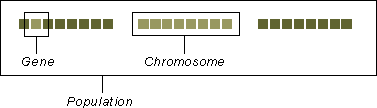
\includegraphics[width=10cm]{gene.png}
\end{center}
\caption{Grafična predstavitev populacije, kromosoma in gena}
\label{pic1}
\end{figure}

Uspešnost teh rešitev nato izmerimo z funkcijo uspešnosti, v nadaljevanju označene z kratico FF (Fitness Function), katera sprejme kot parameter posameznika, oziroma njegov kromosom, in nam pove kako dobro ta posameznik rešuje naš problem. Funkcija v kontekstu evolucije predstavlja posameznikovo zmožnost tekmovati z ostalimi posamezniki populacije. Da bodo GA delali pravilno predpostavimo, da bodo posmezniki z visoko vrednostjo FF proizvedli posameznike, katerih vrednost FF bo večja od staršev. Pri tem upoštevamo, da posmezniki z visokimi vrednostmi FF se bodo tudi večkrat razmnoževali kot tisti z manjšimi vrednostmi FF in s tem izboljšali prihodnje generacije. Torej cilj GA je najti posameznika z največjo možno vrednostjo FF. To doseže z izmenjavanjem genov posameznikov glede na vrednost FF.
\subsection{Algoritem}
Kot je omenjeno zgoraj, GA skozi potek delovanja ne spreminja velikosti. Za vsakega posameznika hranimo njihov kromosom in vrednost FF. Prvo generacijo inicijaliziramo naključno, torej vsak posameznik dobi naključno generirani kromosom. Nato tem posameznikom izmerimo vrednost FF. Glede na vrednost FF nato posameznike razmnožimo. Posamezniki z vsikimi vrednostmi FF dobijo več priložnosti za razmnoževanje kot posamezniki z nizkimi vrednostmi FF. Kromosome staršev križimo in s tem dobimo kromosome Potomcev. Potomci, ki nastanejo kot rezultat križanja, nosijo karakteristike staršev (mešanico genov staršev). Ker pri razmoževanju dobimo nove posameznik moramo velikost populacijo prilagoditi prejšni velikosti. To najlažje naredimo tako, da se znebimo najslebših posameznikov (najnižje vrednosti FF). S tem omogočamo, da se zaporedne generacije izboljšujejo. Da se populacij ne bi vjela v lokalni maksimum FF posameznike, z majhno vrjetnostjo, tudi mutiramo. Mutiramo jih tako, da jim naključno spremenimo neke gene. Ta postopek nato ponavljamo za neko fiksno število generacij ali pa dokler ne dobimo posameznika, ki je dovolj dober.\newpage Delovanje algoritma lahko opišemo z naslednjo pseudo kodo:
\begin{lstlisting}
1. Nakljucno inicializirajo populacjo(t)
2. Doloci vrednosti funkcije uspesnosti populacije(t)
3. Ponavljaj
	1. Izberi starse, za krizanje, iz populacije(t)
	2. Z izbranimi starsi izvedi krizanje in s tem izdelaj populacijo(t+1)
	3. Populacijo(t+1) mutiramo
	4. Doloci vrednosti funkcije uspesnosti populacije(t+1)
4. dokler najboljsi posameznik ni dovolj dober
\end{lstlisting}
\subsection{Inicializacija}
Kot smo omenili prej, inicializiramo populacijo naključno, ponavadi omejeno na določeno območje. Pri tem prilagodimo velikost populacije kompleksnosti iskalne domene.
\subsection{Izbor staršev}
Starše za razmnoževanje se izbere na podlagi vrednosti FF. Torej posamezniki z visokimi vrednostmi bodo imeli večjo vrjetnost biti izbrani za starše. Najbolj enostaven način je, da posameznike uredimo glede na vrednost FF in izberemo N  najboljših. N je število staršev. Težava pri tem je, da izbor staršev ni proporcionalen glede na vrednost FF ampak samo glede na zaporedno mesto v urejeni populaciji. Metode, ki upoštevata to sta izbor z ruletnim kolesmo in univerzalno stohastično vzorčenje.
\subsubsection{Izbor z ruletnim kolesmo}
Izbor z ruletnim kolesmo, v nadaljevanju označen z kratico RWS(roulette-wheel selection), znan tudi kot vrednost upsešnosti proporcionalni izbor (fitness proportionate selection), je metoda izbiranja staršev, ki izbira posameznike proporcionalno glede na vrednost FF. Starše izbira z naključnim vzorčenjem prostora, ki vsebuje normiran nabor vrednosti FF posameznikov populacije. Ta prostor dobimo tako, da vrednosti FF uredimo po velikosti in jih normiramo tako, da je seštevek vseh enak 1. Nato, na intervalu od 0 do 1, izberemo naključno število. Starša izberemo glede na to v čigav interval to število nato pade~\ref{picRWS}. To nato ponavljamo dokler ne dobim željeno število staršev~\ref{picRWS2}.
\begin{figure}[H]
\begin{center}
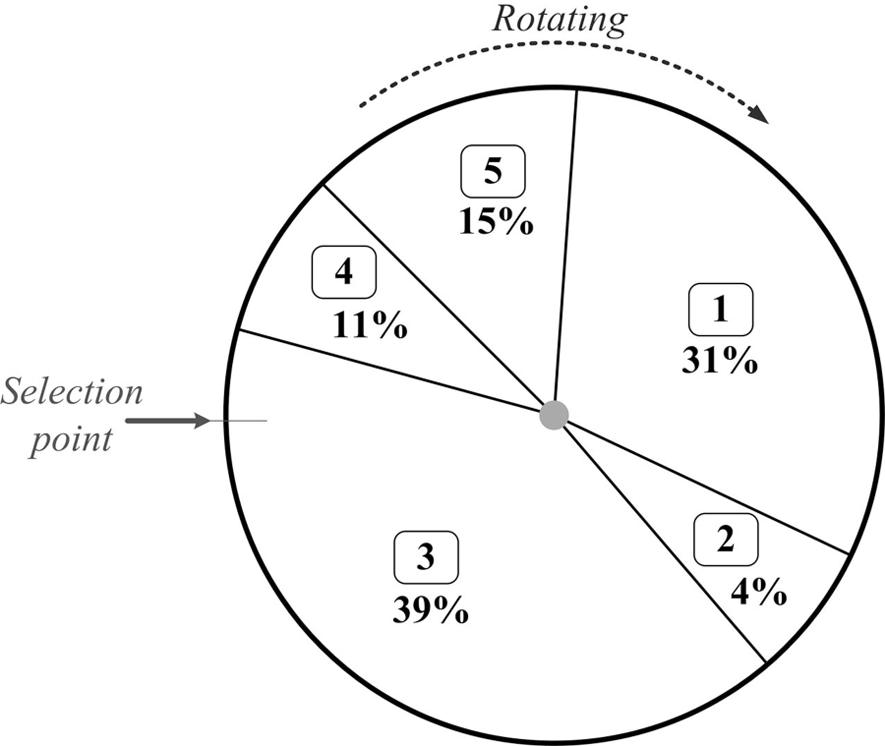
\includegraphics[width=10cm]{roullett.png}
\end{center}
\caption{Primer enega vzorca RWS}
\label{picRWS}
\end{figure}

\begin{figure}[H]
\begin{center}
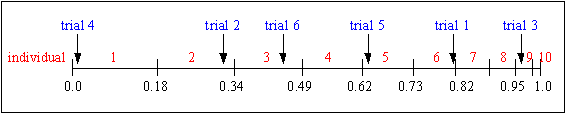
\includegraphics[width=10cm]{roullette2.png}
\end{center}
\caption{Primer celotnega izbora RWS}
\label{picRWS2}
\end{figure}

Algoritem izbira starše proporcionalno na vrednosti FF, vendar težava se pojavi, če en posamezni zavzema večji del celotnega intervala in se tako zgodi, da ostali posamezniki nikoli niso izbrani.
\subsubsection{Univerzalno stohastično vzorčenje}
Univerzalno stohastično vzorčenje, v nadaljevanju označeno z kratico SUS (Stochastic universal sampling), želi popraviti težave, ki so se pojavile pri algoritmu RWS. Vzorčni prostor pripravi na enak način kot pri RWS. Težavo RWS reši z enakomernim vzorčenjem prostor od naključne točke naprej. To da možnost tudi šibkejšim posameznikom, da so izbrani za razmnoževanje. Prvo izbere naključno točko, na intervalu od 0 do 1/N, kjer bo začel vzorčenje. Ta točka predstavlja prvi vzorec. Nato naredi še N-1 vzorcev, vsak zamaknjen za 1/N od prejšnjega. Starše nato izberemo glede na to v čigav interval te vzorci padejo~\ref{picSUS}.
\begin{figure}[H]
\begin{center}
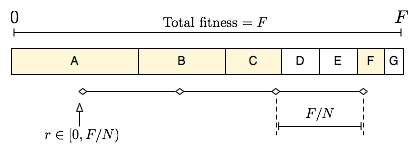
\includegraphics[width=10cm]{Statistically_Uniform.png}
\end{center}
\caption{Primer SUS}
\label{picSUS}
\end{figure}

\subsubsection{Elitizem}
Elitizem pomeni, da vsaki zaporedni generaciji dodamo nekaj najboljših prejšnje generacije. Pri GA, pri katerih zaporedne generacije ne nujno pomenijo boljše posamznike, izboljša elitizem, iskanje saj so najboljši kromosomi vedno prisotni. Elitizem tako nudi pospešitev pri iskanju. Kritike elitizma so predvsem v tem, ker niso skladne z principi naravne selekcije, katere GA simulirajo.

\subsection{Genetski operatorji}
Naslednji korak je, da iz izbranih staršev naredimo novo generacijo. To naradimo z pomočjo genetskih operatorjev: Križanja in mutacija.
\subsubsection{Križanje}
Križanje je postopek, ki združi koromosome dveh ali več staršev v kromosom otroka. Križanje mora biti prilagojeno glede na tip kromosoma. Torej pri kromosom v obliki permutacije moramo paziti da križanje ne bodo dodali enakih števil, pri kromosomu v obliki drevesa naredimo križanje tako da izmenamo veje dreves in tako naprej. V nadaljevanju bo opisanih nekaj metod kako križati kromosomo v obliki vektorja števil saj so najbolj pogosti tipi kromosomov.
Najbolj enostaven način križanja je križanje po eni točki~\ref{picOnePoint}. Prvo določimo eno točko, ki razdeljuje kromosom na dva dela. Pri tem načinu križanja dobimo dva otroka. Prvi otrok dobi levi del kromosoma prvega starša in desni del kromosoma drugega starša.
\begin{figure}[H]
\begin{center}
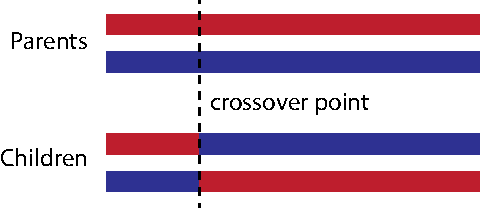
\includegraphics[width=10cm]{OnePointCrossover.pdf}
\end{center}
\caption{Primer križanja po eni točki}
\label{picOnePoint}
\end{figure}
Najlažja izboljšava je tega je da dodamo več točk in za vsako točko spremenimo čigave gene prejme. Te algoritmi se imenijo gleda na število točk, ki jih uporabimo. Torej če imamo 2 točke se bo križanje imenovano križanje po dveh točkah~\ref{picTwoPoint}.
\begin{figure}[H]
\begin{center}
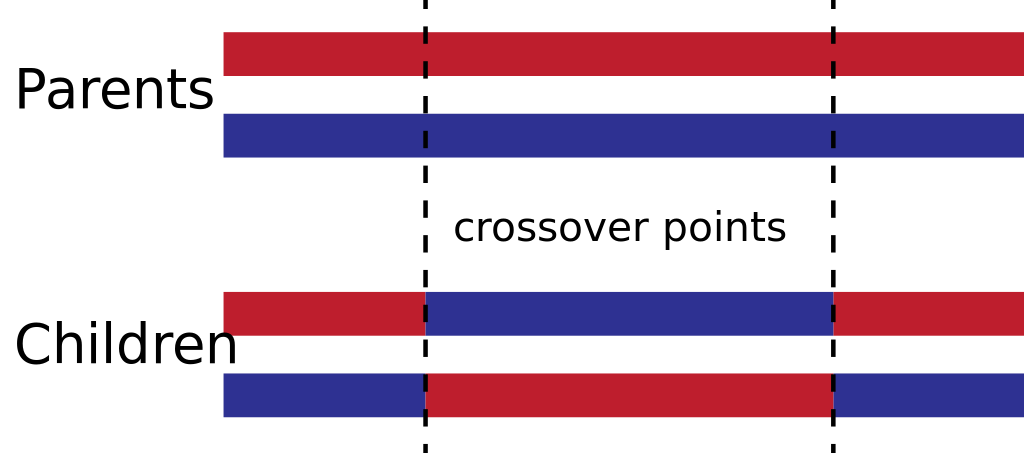
\includegraphics[width=10cm]{TwoPointCrossover.png}
\end{center}
\caption{Primer križanja po dveh točkah}
\label{picTwoPoint}
\end{figure}
Težava pri takem načinu križanja je, da se geni izmenjujejo vedno po istem ključu to težavo rešuje enakomerno križanje~\ref{picUni}. Pri enakomernem križanju uporabljamo fiksno mešalno  vrjetnost, ki nam pove ali se bo gen izmenjav. Torej za vsak gen generiramo naključno število, na interavlu od 0 do 1, in če je ta večja od mešalne vrjetnosti se gena izmenjata, če je manjša se ne. Torej z mešalno vrjetnostjo 0.5 se bo okoli 50\% genov izmenjalo.
\begin{figure}[H]
\begin{center}
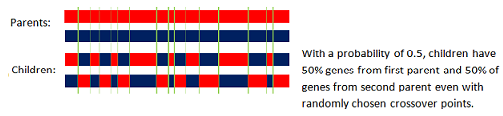
\includegraphics[width=10cm]{UniformCrossover.png}
\end{center}
\caption{Primer enakomernega križanja}
\label{picUni}
\end{figure}
Za križanje lahko uporabimo tudi več staršev in stem izboljšamo tudi kvaliteto dobljenega kromosoma. To najlažje naredimo tako, da za vsak gen še naključno izberemo starše katerih gene bomo križali.
\subsubsection{Mutacije}
GA se ujemajo v lokalne maksimum, to bojujemo z mutacijo. Po tem ko smo starše križali je dobro, da dobljene otroke še mutiramo. To pomeni, naključno spremenimo določene gene v kromosomu. To lahko naredimo fiksno, tako da se vedno isti gen spremni, ali pa naključno, podobno kot pri univerzalnem križanju. Ker se gen naključno spremeni lahko dobimo posameznika, ki se ne nahaja v enaki okolici iskalne domene kot ostali posamezniki populacije. Z nadaljnim izvajanjem GA se lahko izkaže, da se te posamezniki nahajajo bližje globalnemu maksimumu kot kromosomi pred mutacijo.
\subsection{Prekinitev}
Kako vediti kdaj algoritem prekiniti? Najbolj osnovna metoda prekinitve je, da algoritem prekinemo po nekem fiksnem številu generaciji. Pri preprostejših problemih, algoritem hitro konvergira proti neki rešitvi, pri zahtevnejših ne. Zato je dobro slediti spreminjanju najboljšega kromosoma. Če se po nekaj generacijah ne spremeni potem lahko algoritem prekinemo. V nekaterih primerih želimo dobiti le dovolj dobro rešitev. V tem primeru postavimo prag vrednosti FF in če najboljši posameznik preseže ta prag potem lahko algoritem prekinemo.
\subsection{Prednosti in slabost}
Prednosti GA so, da so bolj robustni in manj prostorsko zahtevni kot drugi podobni iskalni algoritmi (naprimer linearno programiranje, iskanje v globino, iskanje v širino...). Nudijo tudi prednosti pri optimizaciji visoko prostorskih, več modelnih in visko dimenzjonalnih problemov, saj prostor ne preiskujejo izčrpno. Težava GA je, da se ujamejo v lokalne maksimume. Za reševanje visoko dimenzijonalnih večmodelnih problemov rabimo enako kompleksno FF, te funkcije so ponavadi zelo časovno zahtevne, zato za zaporedno računanje te funkcije porabimo veliko časa. Težava je tudi, da se z kompleksnostjo problema veča tudi iskalna domena in to zahteva tudi večje populacije, ki pa zahtevajo temu primerno večjo število izračunov FF. Uporabljati jih tudi ne morem na dinamičnih podatki, saj bi se z podatki spreminjala tudi iskalna domena in s tem tudi maksimumi FF.
\chapter{Implementacija}
\section{Generiranje dreves}
\section{Genetski algoritimi}
\chapter{Rezultati}
\begin{thebibliography}{99}
\addcontentsline{toc}{chapter}{Literatura}
\bibitem{lf} L.\ Fortnow, ``Viewpoint: Time for computer science to grow up'',
{\it Communications of the ACM}, št.\ 52, zv.\ 8, str.\ 33--35, 2009.

\bibitem{dk1} D.\ E.\ Knuth, P. Bendix. ``Simple word problems in universal algebras'', v zborniku: Computational Problems in Abstract Algebra (ur.\ J. Leech), 1970, str.\ 263--297.

\bibitem{lat} L.\ Lamport. \textit{LaTEX: A Document Preparation System}. Addison-Wesley, 1986.

\bibitem{bib} O.\ Patashnik (1998) \BibTeX{}ing.
[Online]. Dosegljivo:\\ http://ftp.univie.ac.at/packages/tex/biblio/bibtex/contrib/doc/btxdoc.pdf. [Dostopano 18. 9. 2014].

\bibitem{pdfa} 
PDF/A.
[Online]. Dosegljivo:\\ http://en.wikipedia.org/wiki/PDF/A. [Dostopano 19. 9. 2014].

\bibitem{licence} GNU General Public Licence. [Online]. Dosegljivo:\\ https://www.gnu.org/copyleft/gpl.html. [Dostopano 20. 9. 2014].
\end{thebibliography}
\end{document}

